% Tiros–Brownsville technical report. Built on model v1.0 (final) (model/Tiros_Brownsville_Model.xlsx).
% Compile: cd report && latexmk -pdf tiros_brownsville_report.tex   (figures: see README.md)
% Numbers in the text are typed in: check them against the model's Summary and Model tabs after any model change.
\documentclass[11pt,letterpaper]{article}
\usepackage[T1]{fontenc}
\usepackage[utf8]{inputenc}
\usepackage[scaled=0.92]{helvet}
\renewcommand\familydefault{\sfdefault}
\usepackage{sansmath}\sansmath
\usepackage[margin=2.1cm, top=2.3cm, bottom=2.3cm]{geometry}
\usepackage{xcolor}
% Team palette (docs/style-guide.md)
\definecolor{ink}{HTML}{26313A}
\definecolor{oxide}{HTML}{1E5245}
\definecolor{sand}{HTML}{F6EFDF}
\definecolor{band}{HTML}{F3F5F2}
\definecolor{muted}{HTML}{6B7780}
\definecolor{rule}{HTML}{C9CFC9}
\definecolor{amber}{HTML}{9A6A14}
\definecolor{brick}{HTML}{A33B2B}

\usepackage[version=4]{mhchem}
\usepackage{graphicx}
\usepackage{booktabs, tabularx, array, makecell, colortbl}
\usepackage{enumitem}
\usepackage{titlesec}
\usepackage{tocloft}
\usepackage{fancyhdr, lastpage}
\usepackage[skip=4pt, font=small, labelfont={bf,color=oxide}]{caption}
\usepackage{microtype}
\usepackage{float}
\usepackage[section]{placeins}% floats never cross into the next section
\usepackage{xurl}
\usepackage[colorlinks=true, linkcolor=oxide, urlcolor=oxide, citecolor=oxide, linktoc=all, bookmarksnumbered=true,
            pdftitle={Technical Assessment and Conceptual Process Design: Tiros-Brownsville}]{hyperref}

% ---------- look: oxide green headings, thin rules (docs/style-guide.md)
\color{ink}
\titleformat{\section}{\large\bfseries\color{oxide}}{\thesection}{0.6em}{}[\vspace{-2pt}{\color{rule}\titlerule}]
\titleformat{\subsection}{\normalsize\bfseries\color{oxide}}{\thesubsection}{0.6em}{}
\titlespacing*{\section}{0pt}{12pt}{6pt}
\titlespacing*{\subsection}{0pt}{9pt}{3pt}
\usepackage{needspace,etoolbox}
\pretocmd{\subsection}{\needspace{4\baselineskip}}{}{}% keep a heading with at least a few lines of its text
\pretocmd{\section}{\needspace{6\baselineskip}}{}{}
\setlength{\parindent}{0pt}
\setlength{\parskip}{5pt}
\setlist{itemsep=1pt, topsep=2pt, leftmargin=1.3em}
\renewcommand{\arraystretch}{1.18}
\arrayrulecolor{ink!70}
\newcolumntype{L}{>{\raggedright\arraybackslash}X}
\pagestyle{fancy}
\fancyhf{}
\renewcommand{\headrulewidth}{0pt}
\fancyhead[L]{\footnotesize\color{muted}Tiros--Brownsville: technical assessment and conceptual process design}
\fancyhead[R]{\footnotesize\color{muted}Final report \textperiodcentered{} November 2026}
\fancyfoot[C]{\footnotesize\color{muted}Page \thepage\ of \pageref{LastPage}}
\fancypagestyle{plain}{\pagestyle{fancy}}% the contents page uses the same header and footer

% ---------- a gentle table of contents: sections and subsections, light dotted leaders
\renewcommand{\cfttoctitlefont}{\Large\bfseries\color{oxide}}
\renewcommand{\cftsecfont}{\bfseries\color{ink}}
\renewcommand{\cftsecpagefont}{\bfseries\color{ink}}
\renewcommand{\cftsubsecfont}{\color{muted}}
\renewcommand{\cftsubsecpagefont}{\color{muted}}
\renewcommand{\cftsecleader}{\color{rule}\cftdotfill{\cftdotsep}}
\renewcommand{\cftsubsecleader}{\color{rule}\cftdotfill{\cftdotsep}}
\setlength{\cftbeforesecskip}{7pt}
\setlength{\cftbeforetoctitleskip}{0pt}
\setlength{\cftaftertoctitleskip}{12pt}
\setcounter{tocdepth}{2}

% ---------- trust labels (the brief's three categories)
\newcommand{\known}{\textit{\textcolor{oxide}{Known}}}
\newcommand{\assume}{\textit{\textcolor{amber}{Assumption}}}
\newcommand{\test}{\textit{\textcolor{brick}{Needs testing}}}
\newcommand{\usd}[1]{US\$#1}
\newcommand{\tio}{\ce{TiO2}}
\newcommand{\tocomplete}[1]{\textit{\textcolor{muted}{#1}}}
% clickable cross-references that also give the page: \sref{label} -> "Section 4.9 (p. 12)"
\newcommand{\sref}[1]{\hyperref[#1]{Section~\ref*{#1} (p.~\pageref*{#1})}}
\newcommand{\tref}[1]{\hyperref[#1]{Table~\ref*{#1}}}
\newcommand{\fref}[1]{\hyperref[#1]{Figure~\ref*{#1}}}

\begin{document}

% ======================================================================= TITLE
\begin{titlepage}
\thispagestyle{empty}
\vspace*{2.2cm}
{\color{oxide}\rule{\linewidth}{1.2pt}}\\[10pt]
{\Huge\bfseries\color{oxide} Technical Assessment and\\[4pt] Conceptual Process Design}\\[14pt]
{\Large Titanium and rare-earth recovery from Tiros ore\\[3pt] Brownsville, Texas}\\[8pt]
{\color{oxide}\rule{\linewidth}{0.6pt}}

\vspace{1.4cm}
{\small\color{muted} PREPARED FOR}\\[2pt]
{\large Resouro Strategic Metals Inc.}\\[2pt]
Colorado Impact Challenge, McNeil Innovation Center

\vspace{0.9cm}
{\small\color{muted} PREPARED BY}\\[4pt]
\begin{tabular}{@{}ll@{}}
Jacob Dold & University of Colorado Boulder\\
Lukas Hirschmann & Colorado School of Mines\\
Mathias Bauer & Colorado School of Mines\\
\end{tabular}

\vspace{0.9cm}
{\small\color{muted} COMPANION FILE}\\[2pt]
Editable model: \texttt{Tiros\_Brownsville\_Model.xlsx} (version 1.0, November 2026)

\end{titlepage}

% ======================================================================= CONTENTS
\setcounter{page}{2}% the title page is page 1
\thispagestyle{fancy}
\tableofcontents
\newpage

% ======================================================================= SUMMARY
\section*{Summary}\addcontentsline{toc}{section}{Summary}\label{sec:summary}

\textbf{What this report covers.} The challenge brief from Resouro~\cite{brief} asked for four deliverables, and the report is built around them:
\begin{enumerate}[itemsep=0pt]
\item a \textbf{technology and process assessment} of the ways to turn Tiros ore into a titanium dioxide (\tio) concentrate and a mixed rare-earth carbonate (MREC) (\sref{sec:tech});
\item a \textbf{conceptual process flow} at about 5,000 tonnes a month of ore, showing where later titanium and rare-earth modules could be added (\sref{sec:pfd});
\item a \textbf{technology decision matrix} and the recommended initial Brownsville configuration (\sref{sec:matrix});
\item a \textbf{preliminary mass, economic and development model}, delivered as an editable Excel workbook (\sref{sec:model}), with the highest-priority tests in the \hyperref[sec:conclusion]{Conclusion}.
\end{enumerate}

\textbf{The question.} How could Tiros ore be turned into \tio\ concentrate and MREC at Brownsville, Texas, at about 5,000 tonnes a month of run-of-mine ore (ore as it comes out of the pit), and what must be tested before a pilot plant?

\textbf{Outputs at 5,000 t/month.} Using the processing route in Resouro's July 2026 Preliminary Economic Assessment (PEA)~\cite{pea}, 5,000 t/month of ore would yield about 424 t/month of coarse \tio\ concentrate, 479 t/month of fine \tio\ concentrate and 52 t/month of rare-earth carbonate. Most of the ore, about 81\%, leaves as residue. These figures are the PEA's design values scaled down, not test results.

\textbf{The three cases.} Every case processes the same 5,000 t/month of Tiros ore with the same technology. They differ only in where the steps happen:
\begin{itemize}
\item \textbf{Case 1, Brazil:} all processing at the Tiros mine site in Brazil, as the PEA designs it. The concentrates and the carbonate are sold.
\item \textbf{Case 2, Texas:} the ore is prepared and roasted in Brazil, and the roasted material is shipped to Brownsville, where the acid steps that make the fine \tio\ concentrate and the carbonate take place.
\item \textbf{Case 3, MREC processing Texas:} all processing in Brazil as in Case 1; the finished carbonate is then shipped to Brownsville and separated into individual rare-earth oxides, which sell for more.
\end{itemize}

Each case is valued at two prices for sulfuric acid, the largest bought reagent after caustic soda: the PEA's \emph{normal} price, and the \emph{2026 crisis} price after this year's global acid shortage, about 2.5 times higher.

\textbf{What we found.}
\begin{itemize}
\item \textbf{The PEA's processing route is the right technical basis.} It is the only route with test evidence on Tiros ore. The main unknown is not which technology to use but whether the final steps, which turn the acid liquor into saleable products, work on real Tiros material. They have never been run.
\item \textbf{Keeping all processing in Brazil is the strongest case.} It is the only case with positive value at 5,000 t/month, though only modestly, and it turns negative at 2026 crisis acid prices.
\item \textbf{Moving the acid steps to Texas costs more than it saves.} Case 2 has to ship tens of thousands of tonnes a year of roasted material, run a second site, and dispose of most of that material as residue in Texas.
\item \textbf{Separating Tiros's carbonate in Brownsville does not earn back its plant.} Tiros's rare earths are mostly the lower-value light ones, so separating them adds little value compared with the cost of a separation plant, estimated from Aclara Resources' comparable plant~\cite{aclara}.
\item \textbf{More ore helps every case, and the ranking holds.} Value grows much faster than tonnage, because staff, overheads and much of the build cost do not grow in step (\tref{tab:scale}).
\end{itemize}

\begin{figure}[H]
\centering
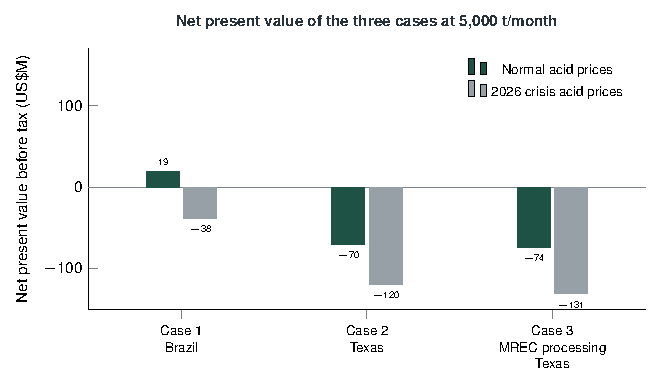
\includegraphics[width=0.78\linewidth]{figures/fig_results.pdf}
\caption{Net present value before tax (today's value of future profit, minus the build cost; 8\% discount rate, 20 years) of the three cases at 5,000 t/month. Summary tab of the model.}\label{fig:results}
\end{figure}

\begin{table}[H]
\centering\small
\caption{Net present value as more Tiros ore is processed, US\$ millions, normal acid prices. In each row, all three cases process the same amount of Tiros ore (Model tab, section F).}\label{tab:scale}
\begin{tabularx}{\linewidth}{@{}Lrrr@{}}
\toprule
\textbf{Tiros ore processed (t/month)} & \textbf{Case 1 Brazil} & \textbf{Case 2 Texas} & \textbf{Case 3 MREC Texas}\\
\midrule
5,000 (the challenge brief) & 19 & $-$70 & $-$74\\
10,000 & 86 & $-$46 & $-$22\\
20,000 & 233 & 18 & 107\\
30,000 & 389 & 93 & 252\\
41,667 (the PEA's full design size) & 575 & 188 & 431\\
\bottomrule
\end{tabularx}
\end{table}

\textbf{Recommendation.} Process Tiros ore fully in Brazil to begin with, and keep Brownsville for later downstream modules once more ore and better prices make them pay (\sref{sec:recommend}). The next step is a short list of tests, led by an end-to-end test of the final liquor-to-product steps (\hyperref[sec:conclusion]{Conclusion}).

% ======================================================================= 1
\section{Technology and Process Assessment}\label{sec:tech}

\textbf{Tiros} is Resouro's titanium and rare-earth project in Minas Gerais, Brazil: a near-surface, intensely weathered deposit. The ore is fine (about 87\% of the rare earths sit in material finer than 53~micrometers), the titanium is mostly in the mineral anatase, the rare earths are in hard-to-leach phosphate minerals, and iron and aluminum are abundant (PEA Sections 7 and 13; Barnard et al.~\cite{barnard}). The July 2026 PEA~\cite{pea} designs a 500,000 t/yr plant around these properties and is our primary source.

\subsection{Technologies by process step}\label{sec:steps}
\tref{tab:tech} compares the options at each step. ``Tiros evidence'' describes what has been shown on Tiros material.

\begin{table}[H]
\centering\scriptsize
\caption{Processing technologies for Tiros ore, step by step. \textbf{Bold} = the PEA's choice, used in the model.}\label{tab:tech}
\begin{tabularx}{\linewidth}{@{}p{2.2cm}p{4.6cm}p{4.2cm}L@{}}
\toprule
\textbf{Step} & \textbf{Options} & \textbf{Tiros evidence} & \textbf{Main risk}\\
\midrule
Feed preparation & \textbf{Scrubbing, screening at 300 and 75\,\textmu m, rod mill on oversize}; desliming (rejecting ultrafines) & Size splits on three samples (BK09, BK11, BK19) & Desliming would lose rare earths; clay-rich fines are hard to thicken and filter\\
Coarse titanium upgrading & \textbf{Magnetic and gravity separation, reduction roast at 600\,\textdegree C, magnetic and electrostatic separation, hydrochloric-acid leach}; flotation & Bench: 76.8\% (BK09) and 79.5\% \tio\ (BK19, no electrostatic stage); PEA design 84.7\% & Lab heavy-liquid separation stands in for industrial gravity separation; anatase market acceptance\\
Fines extraction (titanium and rare earths) & \textbf{Reduction roast, sulfuric-acid bake at 300\,\textdegree C, water leach}; hydrochloric-acid leach; nitric-acid route; ammonium-sulfate leach & Bench: 90.9\% of rare earths and 82.9\% of \tio\ extracted (test MET-53); 72.5\% of rare earths to liquor (BK19) & Hydrochloric and nitric routes extract little or no titanium; ammonium sulfate fails; the bake uses much acid\\
Acid supply & \textbf{Buy 96\% acid}; burn imported sulfur in an acid plant at Tiros; regenerate acid at 600--680\,\textdegree C & PEA assumes about 22\% regenerated: ``conceptual and untested'' (p.272) & Without regeneration, acid use rises from 0.37 to about 0.48 t per t ore; 2026 prices rose 2.5 times\\
Titanium from liquor & \textbf{Hydrolysis by neutralizing with caustic soda} & Not demonstrated on Tiros liquor (p.273) & Rare-earth losses as double sulfates; caustic soda is 40\% of running cost\\
Impurity removal & \textbf{Magnesium hydroxide}; lime & Not tested end to end & Lime is cheaper but forms gypsum and drags rare earths down with it\\
Rare-earth product & \textbf{Carbonate (MREC), precipitated with sodium carbonate}; oxalate; mixed hydroxide & No carbonate yet made and assayed from Tiros liquor & Grade stated as 52\%, 70\% and 95\% in different PEA tables\\
Rare-earth separation (later) & Solvent extraction; continuous ion exchange & None & Needs clean feed and a wastewater route (Case 3)\\
Titanium metal route (later) & Upgrade concentrate, chlorinate to \ce{TiCl4}, Kroll process to sponge & PEA: Tiros products need upgrading first (p.315) & Fine size and silica; no US sponge production in 2025~\cite{usgsti}\\
\bottomrule
\end{tabularx}
\end{table}

\textbf{Reading the table.} At every step the PEA chose the option with the most Tiros evidence, and the alternatives Resouro tested either fail (ammonium sulfate) or recover only one of the two products (hydrochloric and nitric acid). We see no case for a different extraction route at this stage. The real uncertainty lies in steps that have been designed but not run: acid regeneration, titanium hydrolysis, impurity removal and carbonate precipitation on actual Tiros liquor. Those steps carry the rare earths, which are 68\% of revenue in the model.

\subsection{Where the steps happen: three cases}\label{sec:cases}
Brownsville can enter the flowsheet at different points. These define the model's three cases:
\begin{itemize}
\item \textbf{Case 1: Brazil.} Everything at Tiros; the concentrates and carbonate are sold. This is the PEA layout.
\item \textbf{Case 2: Texas.} The fines are roasted at Tiros and shipped as a dry ``calcine'' (roasted powder), about 36,000 t/yr in bulk; everything from the sulfuric-acid bake onward runs in Brownsville.
\item \textbf{Case 3: MREC processing Texas.} As Case 1, then the finished carbonate, about 620 t/yr in bags in containers, is shipped to a rare-earth separation plant in Brownsville, which sells the separated oxides.
\end{itemize}

\textbf{Why Case 2 costs more.} About 80\% of the calcine shipped to Texas ends up as residue, so Case 2 pays to ship roughly 36,000 t/yr across the ocean mostly to landfill about 29,600 t/yr of it in Texas. It also needs a second site with its own staff and overheads, and a permit for the plant's sodium-sulfate wastewater, the issue that stalled Lynas's rare-earth plant at Seadrift, Texas~\cite{lynas}. Cheaper Texas reagents save far less than these costs add.

% ======================================================================= 2
\section{Conceptual Brownsville Process Flow}\label{sec:pfd}

\subsection{Pathway at 5,000 t/month}\label{sec:pathway}
\fref{fig:pfd} shows the pathway from Tiros ore through feed preparation and beneficiation to the two \tio\ concentrates and the carbonate, at the challenge brief's 5,000 t/month; \tref{tab:streams} lists the main streams. The red dashed box marks the steps that move to Brownsville in Case 2; the green box shows the Brownsville separation plant of Case 3. Grey dashed boxes are later modules.

\begin{figure}[H]
\centering
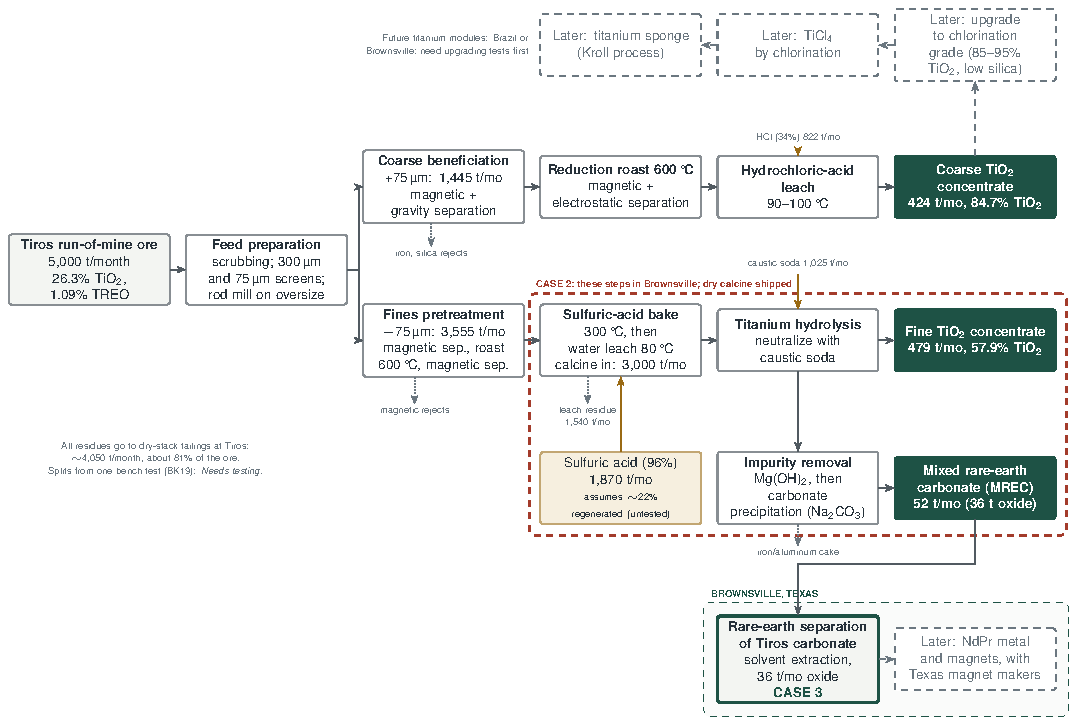
\includegraphics[width=\linewidth]{figures/fig_pfd.pdf}
\caption{Conceptual process flow at 5,000 t/month of Tiros run-of-mine ore. Stream values from the model (Model tab, part B), divided by 12. Green boxes are products; sand boxes are bought reagents; dotted arrows are residues.}\label{fig:pfd}
\end{figure}

\begin{table}[H]
\centering\small
\caption{Main streams at 5,000 t/month (dry tonnes; the PEA does not give ore moisture).}\label{tab:streams}
\begin{tabularx}{\linewidth}{@{}Lrlp{2.3cm}@{}}
\toprule
\textbf{Stream} & \textbf{t/month} & \textbf{Basis} & \textbf{Label}\\
\midrule
Run-of-mine ore & 5,000 & Challenge brief & \known\\
Coarse fraction (+75\,\textmu m) to the coarse circuit & 1,445 & 28.9\% of ore, PEA bench test BK19 & \test\\
Fine fraction ($-$75\,\textmu m, natural and ground) & 3,555 & 71.1\% of ore, PEA bench test BK19 & \test\\
Calcine to the acid bake (shipped in Case 2) & 3,000 & 60.0\% of ore, PEA bench test BK19 & \test\\
Sulfuric acid, 96\% & 1,870 & PEA p.276; includes untested regeneration & \test\\
Caustic soda & 1,025 & PEA p.341 & \known\\
Hydrochloric acid, 34\% & 822 & PEA p.341 & \known\\
Coarse \tio\ concentrate (84.7\% \tio) & 424 & PEA p.275 & \known\\
Fine \tio\ concentrate (57.9\% \tio) & 479 & PEA p.275 & \known\\
Carbonate (MREC) & 52 & Oxide $\div$ 70.3\% oxide content (PEA p.349) & \test\\
\quad of which rare-earth oxide & 36 & 67\% recovery (PEA p.274--275) & \test\\
Residues to tailings (Case 1) & 4,046 & Ore minus products & calculated\\
\bottomrule
\end{tabularx}
\end{table}

\subsection{Where future modules attach}\label{sec:modules}
\begin{itemize}
\item \textbf{Rare-earth separation} attaches to the carbonate stream. It is the only module costed in the model (Case 3, \sref{sec:case3}). It changes nothing upstream, apart from needing a clean, assayed carbonate.
\item \textbf{\ce{TiCl4} and titanium sponge} attach to the coarse concentrate, but only after an upgrading step: chlorinators need about 85--95\% \tio\ with little silica, and the PEA says Tiros's products must be upgraded first (p.315). The fine concentrate (57.9\% \tio, below 20\,\textmu m) is not a chlorination feed. These modules could sit in Brazil or Brownsville; they are described, not costed.
\item \textbf{Rare-earth metal and magnets} attach after separation, with partners. Texas already hosts US magnet makers (MP Materials in Fort Worth, Noveon in San Marcos).
\end{itemize}

% ======================================================================= 3
\section{Technology Decision Matrix}\label{sec:matrix}

\subsection{Method}\label{sec:method}
The extraction technology itself is settled in \sref{sec:tech}: the PEA route is the only one with Tiros evidence, and every case uses it. The most important remaining choice is how the process is configured between Tiros and Brownsville, so the matrix compares the three cases. Each case is scored from 1 (poor) to 5 (strong) on each criterion from the challenge brief, plus economic value from the model. Each score is multiplied by the criterion's weight, and the weighted scores are added up (maximum 5.0). Economic value carries the most weight because it combines most of the measurable criteria; product quality the least, because all three cases make the same titanium products.

\subsection{Decision matrix}\label{sec:matrixtable}
\begin{table}[H]
\centering\small
\caption{Decision matrix for the three cases. Scores 1 (poor) to 5 (strong).}\label{tab:matrix}
\begin{tabularx}{\linewidth}{@{}>{\raggedright\arraybackslash}p{4.0cm}>{\centering\arraybackslash}p{1.2cm}>{\centering\arraybackslash}p{1.3cm}>{\centering\arraybackslash}p{1.3cm}>{\centering\arraybackslash}p{1.7cm}L@{}}
\toprule
\textbf{Criterion} & \textbf{Weight} & \textbf{Case 1 Brazil} & \textbf{Case 2 Texas} & \textbf{Case 3 MREC Texas} & \textbf{Evidence}\\
\midrule
Technical maturity & 10\% & 4 & 3 & 3 & Note below; \tref{tab:tech}\\
Expected recovery & 10\% & 3 & 3 & 3 & \tref{tab:streams}; \tref{tab:mass}\\
Product quality & 5\% & 3 & 3 & 4 & Note below\\
Capital requirements & 10\% & 5 & 4 & 2 & \tref{tab:capex}\\
Operating complexity & 10\% & 4 & 2 & 3 & Note below\\
Energy and reagent requirements & 10\% & 4 & 3 & 3 & \tref{tab:opex}\\
Environmental considerations & 10\% & 3 & 2 & 3 & Note below\\
Scalability & 10\% & 5 & 3 & 4 & \tref{tab:scale}\\
Technical risk & 10\% & 3 & 2 & 2 & Note below\\
Economic value (net present value) & 15\% & 4 & 1 & 1 & \tref{tab:results}; \fref{fig:results}\\
\midrule
\textbf{Weighted total (out of 5.0)} & 100\% & \textbf{3.85} & \textbf{2.50} & \textbf{2.65} & \\
\bottomrule
\end{tabularx}
\end{table}

\textbf{Notes on the scores that rest on judgment.}
\begin{itemize}
\item \textbf{Technical maturity.} Every unit in the PEA flowsheet is used commercially somewhere, so Case 1 scores well, though the full sequence has never run on anatase ore. Case 2 uses the same units but splits them across two continents, with roasted material stored, shipped and reheated in between, which no comparable plant does. Case 3 adds solvent extraction, a mature technology, but at a very small scale and on a carbonate that has never been made.
\item \textbf{Expected recovery.} All three cases use the same process, so recoveries are the same; the 67\% rare-earth recovery is itself unproven. Case 3 loses about 5\% more in separation but sells the rest at a higher value, so it scores the same.
\item \textbf{Product quality.} The titanium concentrates are the same in every case. Case 3 sells separated oxides, which more buyers can use than a mixed carbonate, and which are made in the US.
\item \textbf{Operating complexity.} Case 1 is one site. Case 2 runs two sites that depend on each other through a 36,000 t/yr bulk shipping chain, under two countries' permits. Case 3 also has two sites, but they are loosely linked by a small container flow, and a separation plant has many circuits to run.
\item \textbf{Environmental considerations.} In Case 1 all residue stays in the dry-stack tailings at Tiros, which the PEA already plans. Case 2 moves about 29,600 t/yr of residue and a sodium-sulfate wastewater stream to Texas, where wastewater stopped Lynas's plant, and adds ocean freight. Case 3 adds only the separation plant's own, smaller wastewater stream in Texas.
\item \textbf{Technical risk.} All cases share the untested liquor-to-product steps. Case 2 adds the risk that calcine changes during storage and shipping; Case 3 adds the risk that Tiros carbonate, including its thorium and uranium content, does not meet separation feed requirements.
\end{itemize}

\subsection{Recommended initial Brownsville configuration}\label{sec:recommend}
Case 1 scores highest (3.85 out of 5), well ahead of Cases 3 and 2. It wins on economic value, capital, scalability and simplicity, and it is the only case with positive value at the challenge brief's size. We therefore recommend:
\begin{enumerate}[itemsep=1pt]
\item \textbf{Process Tiros ore fully in Brazil to start}, using the PEA flowsheet (\fref{fig:pfd}), producing coarse and fine \tio\ concentrates and a mixed rare-earth carbonate.
\item \textbf{Do not move the acid steps to Brownsville.} Case 2 scores lowest and loses value at every ore rate tested.
\item \textbf{Keep Brownsville for downstream modules, added in stages.} Rare-earth separation is the natural first Brownsville module, but it should wait until a toll trial of Tiros carbonate with an existing separator shows that separating pays, and until more ore is processed: Case 3 turns positive only above about 12,000 t/month. Rare-earth metal and magnets, and the titanium route (upgrading, \ce{TiCl4}, sponge), follow later with partners.
\end{enumerate}

\subsection{What is known and what still needs testing}\label{sec:known}
Every model input carries one of the challenge brief's three labels: 22 are \known\ (stated in the PEA, the challenge brief or a published fact), 19 are \assume\ (our planning choices, such as reagent prices, freight and the separation-plant costs from Aclara) and 7 are \test. The seven that need testing are the ones the scores above lean on most: the fine and calcine shares of the ore, the 67\% rare-earth recovery (the PEA's economic model uses 80.5\%), the carbonate's oxide content, the acid use including untested regeneration, the safe shipping moisture, and recovery in separation. Thorium and uranium content, wastewater treatment, and whether the fine \tio\ concentrate can be sold are not yet in the model at all.

% ======================================================================= 4
\section{Preliminary Mass, Economic and Development Model}\label{sec:model}

\subsection{Basis and how the model is built}\label{sec:basis}
The model (\texttt{Tiros\_Brownsville\_Model.xlsx}) is an Excel workbook: a Summary tab with the results, an Inputs tab with all 48 inputs, a Model tab with the three cases side by side, and an MREC Texas tab for the separation plant. Sand-colored cells are inputs; everything else is calculated, and each line says how. Every input carries a source and one of the three labels: \known, \assume\ or \test. All three cases are modeled at the same 5,000 t/month of Tiros ore, so they are compared like for like. The PEA's numbers, designed for a plant 8.3 times larger, are scaled down to that rate.

\begin{table}[H]
\centering\small
\caption{Design basis.}\label{tab:basis}
\begin{tabularx}{\linewidth}{@{}p{3.2cm}Lp{2.3cm}@{}}
\toprule
\textbf{Item} & \textbf{Value used} & \textbf{Label}\\
\midrule
Ore processed & 5,000 t/month = 60,000 t/yr in every case, from the challenge brief & \known\\
Ore grade & 26.3\% \tio; 10,852 parts per million total rare-earth oxide (PEA p.267) & \known\\
Process & The PEA flowsheet (PEA Section 17), scaled to 5,000 t/month & \known\ / \test\\
Prices & PEA long-term: \usd{900}/t coarse, \usd{650}/t fine, \usd{57.40}/kg rare-earth basket, 70\% paid for a carbonate & \known\\
Acid price & Normal: \usd{170}/t delivered to Tiros (PEA). 2026 crisis: \usd{430}/t & \known\ / \assume\\
Money & Before tax; 8\% real discount rate and 20-year life, as in the PEA; build costs scaled with the six-tenths rule (cost grows with size to the power 0.6) & \known\ / \assume\\
\bottomrule
\end{tabularx}
\end{table}

\textbf{A caution we carry throughout.} Resouro's Brownsville roadmap warns that its production estimates are extrapolations and that actual Brownsville recoveries must be established through testing~\cite{plan}. Every production figure here is a PEA design value scaled to 5,000 t/month, not a test result.

\subsection{Mass balance and major losses}\label{sec:mass}
\begin{table}[H]
\centering\small
\caption{Yearly mass balance at 5,000 t/month (every case processes the same ore).}\label{tab:mass}
\begin{tabularx}{\linewidth}{@{}Lrrr@{}}
\toprule
 & \textbf{Ore (t/yr)} & \textbf{\tio\ (t/yr)} & \textbf{Rare-earth oxide (t/yr)}\\
\midrule
In the ore & 60,000 & 15,780 & 651\\
To coarse \tio\ concentrate & 5,087 & 5,087$^{a}$ & --\\
To fine \tio\ concentrate & 5,744 & 5,744$^{a}$ & --\\
To carbonate (620 t of carbonate) & 621 & -- & 436\\
\textbf{Lost to residues} & \textbf{48,549} (81\%) & \textbf{4,949} (31\%) & \textbf{215} (33\%)\\
\bottomrule
\end{tabularx}\\[2pt]
{\footnotesize\color{muted} $^{a}$ The PEA's product tonnages and its stated titanium recovery (68.7\%) only agree if the tonnages count the \tio\ inside the concentrates; but the PEA prices them as tonnes of concentrate. The model follows the PEA's own revenue figures. Testing should settle which is meant.}
\end{table}

\tref{tab:relosses} breaks the 215 t/yr of lost rare-earth oxide down by where it goes. The first five lines are measured in the PEA's BK19 bench test (as a share of the rare earths in the ore); the last line is the PEA's design assumption for the steps never tested.

\begin{table}[H]
\centering\small
\caption{Where the rare earths are lost, at 5,000 t/month.}\label{tab:relosses}
\begin{tabularx}{\linewidth}{@{}Lrr@{}}
\toprule
 & \textbf{Share of rare earths in the ore} & \textbf{t/yr of oxide}\\
\midrule
Dissolved in the coarse circuit's hydrochloric-acid leach (not recovered) & 10.7\% & 70\\
Magnetic and gravity rejects & 6.3\% & 41\\
Acid-bake leach residue & 4.5\% & 29\\
Locked in the coarse \tio\ concentrate & 2.3\% & 15\\
Not traced in the test & 3.7\% & 24\\
\quad \textit{Reaching the leach liquor (BK19 test)} & \textit{72.5\%} & \textit{472}\\
Lost between liquor and carbonate (design assumption, untested) & 5.5\% & 36\\
\midrule
\textbf{Total lost} (recovered to carbonate: 67\%, 436 t/yr) & \textbf{33.0\%} & \textbf{215}\\
\bottomrule
\end{tabularx}
\end{table}

\subsection{Operating cost drivers and capital categories}\label{sec:costs}
\begin{table}[H]
\centering\small
\caption{Running cost by line, US\$ millions per year at 5,000 t/month.}\label{tab:opex}
\begin{tabularx}{\linewidth}{@{}Lrrrr@{}}
\toprule
 & \textbf{Case 1} & \textbf{Share of Case 1} & \textbf{Case 2} & \textbf{Case 3}\\
\midrule
Caustic soda & 6.89 & 40\% & 6.40 & 6.89\\
Sulfuric acid (normal year) & 3.81 & 22\% & 3.93 & 3.81\\
Hydrochloric acid (coarse circuit) & 1.97 & 11\% & 1.97 & 1.97\\
Mining, power, maintenance, minor reagents & 1.65 & 10\% & 1.65 & 1.65\\
Staff & 1.24 & 7\% & 4.14 & 1.24\\
Site overheads & 1.00 & 6\% & 2.00 & 1.00\\
Products to market, waste disposal & 0.75 & 4\% & 1.66 & 0.75\\
Case 2: shipping calcine to Brownsville & -- & -- & 3.06 & --\\
Case 3: shipping carbonate to Brownsville & -- & -- & -- & 0.11\\
Case 3: separation plant in Brownsville & -- & -- & -- & 9.64\\
\midrule
\textbf{Total} & \textbf{17.32} & 100\% & \textbf{24.81} & \textbf{27.07}\\
\bottomrule
\end{tabularx}
\end{table}

Three reagents make up 73\% of Case 1's running cost, and caustic soda alone 40\%. Its consumption, 205~kg per tonne of ore, is large for titanium hydrolysis alone and the PEA does not explain its basis, so it is a priority test. Case 2 costs \usd{7.5M}/yr more than Case 1, mostly freight, US staff, a second site and Texas landfill; cheaper Texas caustic soda saves only \usd{0.5M}/yr. Case 3's separation plant costs \usd{9.6M}/yr, more than half of it staff and overheads, against \usd{5.6M}/yr of extra value from selling separated oxides.

The two shipping lines are different flows. Case 2 ships a large bulk tonnage of half-processed ore (calcine) from Tiros to a Brownsville plant that finishes the processing, at about \usd{85}/t. Case 3 ships only the finished carbonate, a few hundred tonnes a year in bags in containers, at about \usd{185}/t from the Brazilian port.

\textbf{How the build cost is split.} The PEA gives a single build cost of \usd{191.2M} for its full-size plant, with no breakdown by area. To cost Case 2, which moves part of the plant to Texas, the model needs to know how much of that cost belongs to the acid (fines) circuit. We assumed 45\%, because that circuit holds most of the process equipment: two of the three kilns, the acid bake, the leach tanks and filters, and the hydrolysis and precipitation steps. The other 55\% covers the mine, site works and the coarse circuit. A breakdown from Resouro would replace this assumption. Both parts are scaled to 5,000 t/month with the six-tenths rule (\tref{tab:capex}). Sustaining capital is the PEA's \usd{5.78} per tonne of ore.

\begin{table}[H]
\centering\small
\caption{Build cost by category, US\$ millions (the PEA's \usd{191.2M} scaled with the six-tenths rule).}\label{tab:capex}
\begin{tabularx}{\linewidth}{@{}Lrrr@{}}
\toprule
 & \textbf{Case 1} & \textbf{Case 2} & \textbf{Case 3}\\
\midrule
Mine, site works and coarse circuit (Brazil; 55\% of PEA cost) & 29.5 & 29.5 & 29.5\\
Acid (fines) circuit (45\% of PEA cost; $\times$1.15 in Texas) & 24.1 & 27.7 & 24.1\\
Brownsville site works, receiving and handling & -- & 12.0 & --\\
Separation plant (from Aclara~\cite{aclara}, scaled to 436 t/yr), after 25\% government support & -- & -- & 52.1\\
\midrule
\textbf{Total} & \textbf{53.6} & \textbf{69.2} & \textbf{105.7}\\
\bottomrule
\end{tabularx}
\end{table}

\subsection{Results for the three cases}\label{sec:results}
\fref{fig:results} in the Summary shows the value of each case at both acid prices; \tref{tab:results} gives the detail.

\begin{table}[H]
\centering\small
\caption{Results at 5,000 t/month, US\$ millions (Summary tab).}\label{tab:results}
\begin{tabularx}{\linewidth}{@{}Lrrr@{}}
\toprule
 & \textbf{Case 1 Brazil} & \textbf{Case 2 Texas} & \textbf{Case 3 MREC Texas}\\
\midrule
Material shipped to Brownsville (t/yr) & 0 & 36,000 calcine & 621 carbonate\\
Solid residue left in Texas (t/yr) & 0 & 29,636 & --\\
Revenue (per year) & 25.8 & 25.8 & 31.5$^{b}$\\
Operating margin (per year) & 7.7 & 0.3 & 3.6\\
Build cost & 53.6 & 69.2 & 105.7\\
\textbf{Net present value, normal acid prices} & \textbf{19.0} & \textbf{$-$70.1} & \textbf{$-$73.6}\\
Net present value, 2026 crisis acid prices & $-$38.2 & $-$119.7 & $-$130.9\\
\bottomrule
\end{tabularx}\\[2pt]
{\footnotesize\color{muted} $^{b}$ Includes \usd{5.6M}/yr of extra value from selling Tiros's rare earths as separated oxides.}
\end{table}

\begin{itemize}
\item \textbf{The challenge brief's 5,000 t/month is marginal on its own.} Case 1 is worth only \usd{19M} and turns negative at 2026 crisis acid prices (\usd{430}/t delivered to Tiros against \usd{170}/t in the PEA).
\item \textbf{Case 2 loses in every test.} Even with every reasonable assumption pulled toward Texas (own acid from Gulf sulfur, on-site residue storage, cheaper freight, fewer and cheaper staff) it stays behind Case 1. Buyers would need to pay 53\% more for US-processed rare earths to close the gap.
\item \textbf{Case 3 trails Case 1 by \usd{93M}:} the separation plant's $-$\usd{92M} and \usd{1M} of freight for the carbonate.
\item \textbf{Processing more ore makes economic sense, and the ranking holds} (\tref{tab:scale} in the Summary; Model tab, section F). Value grows faster than tonnage because staff, overheads and much of the build cost do not grow in step: doubling to 10,000 t/month more than quadruples Case 1's value. Case 1 stays first at every rate tested, up to the PEA's full size. At 2026 crisis acid prices it needs about 20,000 t/month to stay positive.
\end{itemize}

\subsection{Case 3: separating Tiros carbonate, based on Aclara's plant}\label{sec:case3}
No Tiros carbonate has yet been made or separated, so the separation plant in Case 3 is costed from one outside source: \textbf{Aclara Resources' April 2026 technical reports}~\cite{aclara} for its planned separation plant in Louisiana, which will separate carbonate from Aclara's Carina project in Goi\'as, Brazil. \tref{tab:aclara} shows which numbers are Aclara's, scaled to Tiros's much smaller tonnage, and the result.

\begin{table}[H]
\centering\small
\caption{The Case 3 separation plant at 5,000 t/month: inputs, sources and result (MREC Texas tab).}\label{tab:aclara}
\begin{tabularx}{\linewidth}{@{}p{5.2cm}p{3.4cm}L@{}}
\toprule
\textbf{Item} & \textbf{Value} & \textbf{Source}\\
\midrule
Build cost of Aclara's plant & \usd{277M} for 4,378 t/yr of oxide & Aclara, Apr 2026 (excludes working capital)\\
Scaled to Tiros's 436 t/yr & \usd{69.4M}; \usd{52.1M} after 25\% support & Six-tenths rule; support from Aclara's (17\%) and Ucore's (38\%)~\cite{ucore} grants plus the 45X tax credit\\
Running cost & \usd{22.09}/kg separated & Aclara's \usd{10}/kg for reagents and power, plus 45 staff and overheads (our assumption)\\
Recovery in separation & 95\% & Aclara's planned outputs: 93--95\%\\
Extra value from separating & \usd{12.88}/kg of oxide & Element shares from PEA assays (BK09, BK19); PEA prices\\
Extra value needed to break even & \usd{34.25}/kg of oxide & Running cost plus repaying the build cost\\
\midrule
\textbf{Net present value of the plant} & \textbf{$-$\usd{91.5M}} & Against selling the carbonate unseparated\\
\bottomrule
\end{tabularx}
\end{table}

Separating a kilogram of Tiros oxide earns only about \usd{13} more than selling it as carbonate, because neodymium--praseodymium (NdPr) carries most of the value and Tiros has very little dysprosium or terbium (about 0.36\% of its oxide together); lanthanum and cerium, two-thirds of the oxide, are worth under \usd{2}/kg. Aclara's plant is ten times Tiros's size, so its cost per kilogram does not carry over: at Tiros's tonnage, staff and overheads alone are about \usd{12}/kg. Using Aclara's October 2026 redesign (about \usd{494M}) instead would make the plant worth $-$\usd{132M}.

\subsection{Development pathway}\label{sec:pathwaydev}
\begin{table}[H]
\centering\small
\caption{Staged development.}\label{tab:stages}
\begin{tabularx}{\linewidth}{@{}p{3.2cm}Lp{4.6cm}@{}}
\toprule
\textbf{Stage} & \textbf{What} & \textbf{Go ahead when}\\
\midrule
0. Bench (now) & The priority tests in \tref{tab:tests} on representative samples & Liquor-to-product recovery and reagent use confirmed\\
1. Pilot & Continuous pilot of the fines circuit; make carbonate and fine \tio\ samples; toll-separate a carbonate lot & Products meet buyer and separator specifications, including thorium and uranium\\
2. First plant & 5,000 t/month at Tiros, demonstrating the full flowsheet & Pilot recoveries hold; acid supply secured\\
3. Scale-up & Process more Tiros ore, toward the PEA's size (\sref{sec:results}) & First plant runs at design; market for the products\\
4. Brownsville separation & Separation plant for Tiros carbonate (Case 3) & Toll trial and prices show it pays; wastewater route permitted\\
5. Later modules & Metal and magnets with partners; titanium upgrading, \ce{TiCl4} and sponge & Partners commit; upgrading tests succeed\\
\bottomrule
\end{tabularx}
\end{table}

% ======================================================================= CONCLUSION
\section*{Conclusion}\addcontentsline{toc}{section}{Conclusion}\label{sec:conclusion}
Tiros ore can be processed with the route the PEA already designs: physical upgrading of the coarse material, and a sulfuric-acid bake and leach of the fines that carry most of the rare earths. No other route tested on Tiros ore recovers both titanium and rare earths. The gap is demonstration, not technology choice: the final steps that turn the acid liquor into saleable products, and that carry most of the value, have not yet been run on Tiros material.

On where to process, the analysis points one way. Keeping all processing in Brazil is the simplest, cheapest and most valuable configuration. Moving the acid steps to Texas adds shipping, a second site and residue in Texas for little saving. Separating Tiros's own carbonate in Brownsville is a sensible later module, but not yet one that pays. Processing more Tiros ore raises value far more than any change of location, so the way forward is to prove the process, start in Brazil, and grow the tonnage, adding Brownsville modules once tests and prices support them.

\textbf{Highest-priority tests before pilot development.} \tref{tab:tests} lists the five tests that would most change these conclusions, in order. Each is tied to a model input, so results can be entered directly.

\begin{table}[H]
\centering\scriptsize
\caption{The five highest-priority tests.}\label{tab:tests}
\begin{tabularx}{\linewidth}{@{}p{0.3cm}p{3.6cm}p{4.4cm}p{2.6cm}L@{}}
\toprule
\textbf{\#} & \textbf{Test} & \textbf{What it measures} & \textbf{Model input} & \textbf{Decision it supports}\\
\midrule
1 & End-to-end liquor-to-product test on representative fines (bench, then locked cycle) & Titanium hydrolysis, iron and aluminum removal, carbonate precipitation on real liquor; recovery into saleable products & Rare-earth recovery (67\%), carbonate grade, fine \tio\ yield & Whether the rare-earth revenue (68\% of total) is real\\
2 & Acid bake and acid regeneration & Fresh acid needed per tonne of ore, with and without regeneration at 600--680\,\textdegree C & Acid per tonne of ore (0.374) & Acid supply: buy, or build a sulfur-burning plant at Tiros\\
3 & Caustic soda balance & Caustic soda used in hydrolysis and neutralization & Caustic soda per tonne of ore (0.205) & The largest cost line (40\%)\\
4 & Make and assay a test carbonate, including thorium and uranium & Every rare earth, thorium, uranium and impurities; where thorium and uranium end up across residues and products & Element shares (MREC Texas tab); waste disposal & Saleability of the carbonate; permitting; Case 3\\
5 & Variability and mass balance on more samples & Size split, rejects and calcine yield across the deposit, beyond the single BK19 sample & Fines and calcine shares; product yields & Plant sizing at 5,000 t/month and above\\
\bottomrule
\end{tabularx}
\end{table}

% ======================================================================= REFERENCES
\FloatBarrier
\renewcommand{\refname}{References}
\phantomsection\addcontentsline{toc}{section}{References}
{\footnotesize
\begin{thebibliography}{99}\setlength{\itemsep}{-1pt}
\bibitem{pea} K.~Azougarh et al., \emph{NI 43-101 Technical Report and Preliminary Economic Assessment for the Tiros Rare Earths and Titanium Project, Minas Gerais, Brazil}, Norda Stelo for Resouro Strategic Metals Inc., Jul.~2026. \url{https://resouro.com/wp-content/uploads/2026/07/127167.001_Resouro-Tiros_PEA_2026_FINAL_Norda.pdf}
\bibitem{brief} Colorado Impact Challenge, ``Initial Project Information: Tiros--Brownsville'' (the challenge brief), 2026. \url{https://impactconnectcolorado.base44.app/}
\bibitem{plan} Resouro Strategic Metals Inc., ``Tiros Brownsville Plan,'' 21 Sep.~2026, as cited in the challenge brief.
\bibitem{barnard} K.~R.~Barnard et al., ``Processing anatase ores for pigment production,'' \emph{Hydrometallurgy}, vol.~185, pp.~226--237, 2019. \href{https://doi.org/10.1016/j.hydromet.2019.02.006}{doi:10.1016/j.hydromet.2019.02.006}
\bibitem{usgsti} U.S. Geological Survey, ``Titanium and titanium dioxide,'' \emph{Mineral Commodity Summaries 2026}. \url{https://pubs.usgs.gov/periodicals/mcs2026/mcs2026-titanium.pdf}
\bibitem{lynas} Lynas Rare Earths, \emph{FY26 Annual Report}, ASX, 26 Aug.~2026. \url{https://announcements.asx.com.au/asxpdf/20260826/pdf/0737nx07s3tnf7.pdf}
\bibitem{aclara} Aclara Resources, technical reports on its integrated heavy rare-earth project (Carina, Brazil, and Louisiana separation plant), Apr.~2026. \url{https://www.newswire.com/news/aclara-announces-results-from-technical-reports-on-its-integrated-heavy-rare}
\bibitem{ucore} Ucore Rare Metals, engineering report for the Louisiana Strategic Metals Complex, May 2026. \url{https://ucore.com/ucore-engineering-report-drives-optimized-commercial-deployment-plan-for-louisiana-strategic-metals-complex/}
\end{thebibliography}}

\end{document}
